\chapter{Fudamentação Teórica}
\label{fundamentacao}

Neste capítulo, são apresentados os conceitos e técnicas essenciais para desenvolver esta pesquisa. Na Seção \ref{fundamentacao:ageis}, é realizada uma apresentação do que são metodologias ágeis e quais os seus princípios. Na Seção \ref{fundamentacao:redes}, aborda-se a temática de Redes Bayesianas e alguns conceitos relacionados à essa técnica.

\section{Metodologias Ágeis}
\label{fundamentacao:ageis}

Em 2001, o termo "Metodologias Ágeis" tornou-se popular quando um grupo de engenheiros de \textit{software} se reuniu para discutir maneiras de melhorar o desempenho em seus projetos, levando em consideração a crescente taxa de mudanças de requisitos e expectativas dos clientes. Apesar do fato desses engenheiros utilizarem práticas diferentes, um pequeno conjunto dessas práticas e princípios parecia ser comum \cite{williams}. O resultado dessa união foi a criação da \textit{Agile Alliance} e do Manifesto ágil \cite{manifesto}.

Desse dia em diante, são consideradas Metodologias Ágeis aquelas que cumprem com os valores expressados no Manifesto ágil: indivíduos e interações entre eles mais que processos e ferramentas; \textit{software} em funcionamento mais que documentação abrangente; colaboração com o cliente mais que negocioção de contratos; e responder à mudanças mais que seguir um plano. Além desses valores, no Manifesto ágil são elencados doze princípios para guiar equipes ágeis:

\begin{itemize}
 \item Satisfazer o cliente através da entrega contínua e adiantada de \textit{software} com valor agregado;
 \item Mudanças nos requisitos são bem-vindas, mesmo tardiamente no desenvolvimento. Processos ágeis tiram vantagem das mudanças visando vantagem
competitiva para o cliente;
 \item Entregar frequentemente \textit{software} funcionando, de poucas semanas a poucos meses, com preferência à menor escala de tempo;
 \item Pessoas de negócio e desenvolvedores devem trabalhar diariamente em conjunto por todo o projeto;
 \item Construa projetos em torno de indivíduos motivados. Dê a eles o ambiente e o suporte necessário e confie neles para fazer o trabalho;
 \item O método mais eficiente e eficaz de transmitir informações para e entre uma equipe de desenvolvimento é através de conversa face a face;
 \item \textit{Software} funcionando é a medida primária de progresso;
 \item Os processos ágeis promovem desenvolvimento sustentável. Os patrocinadores, desenvolvedores e usuários devem ser capazes de manter um ritmo constante indefinidamente;
 \item Contínua atenção à excelência técnica e bom \textit{design} aumenta a agilidade;
 \item Simplicidade - a arte de maximizar a quantidade de trabalho não realizado - é essencial;
 \item As melhores arquiteturas, requisitos e \textit{designs} emergem de equipes auto-organizáveis;
 \item Em intervalos regulares, a equipe reflete sobre como se tornar mais eficazes e então refina e ajusta seu comportamento de acordo.
\end{itemize}

\subsection{Fatores-Chave do Trabalho em Equipe}
\label{fundamentacao:ageis:fatores}

Como forma de elencar os fatores que influenciam o TE de equipes ágeis, foi realizada uma Revisão Literária, adotando características essenciais de Revisões Sistemáticas, para garantir uma maior quantidade de trabalhos relevantes encontrados. Apesar de não seguir o protocolo necessário para realizar uma Revisão Sistemática em Engenharia de \textit{Software} \cite{kitchenham}, adotou-se nessa Revisão Literária duas etapas essenciais de Revisões Sistemáticas.

A primeira fase é a de Seleção de Trabalhos, onde a relevância dos trabalhos para o contexto desta pesquisa foi avaliada com base em seus nos títulos, \textit{abstracts} e palavras-chave. Em seguida, com base nessas propriedades dos trabalhos, os estudos irrelevantes e duplicados são descartados. Depois disso, ocorre a fase de Extração dos Trabalhos, ou Avaliação da Qualidade dos Trabalhos. Nessa fase, os trabalhos considerados relevantes após a fase de Seleção de Trabalhos foram avaliados com base em suas introduções e conclusões, além de suas respectivas qualidades. Assim, são descartados mais alguns trabalhos. Finalmente, as informações relevantes para esta pesquisa foram extraídas dos trabalhos remanescentes.

Para realizar esse processo, os motores de busca selecionados para servir de fonte de trabalhos foram: \textit{ACM}\footnote{\url{http://dl.acm.org/}}, \textit{IEEE}\footnote{\url{http://ieeexplore.ieee.org/Xplore/home.jsp}}, \textit{Scopus}\footnote{\url{http://www.scopus.com/}}, \textit{Science Direct}\footnote{\url{http://www.sciencedirect.com/}} e \textit{Google Scholar}\footnote{\url{https://scholar.google.com.br/}}. Em seguida, foram definidas as \textit{strings} de busca para cada um desses motores. Além disso, foi utilizada a ferramenta \textit{StArt}\footnote{\url{http://lapes.dc.ufscar.br/tools/start_tool}} para auxiliar a gerência das informações referentes aos trabalhos encontrados.

Nesse processo de revisão literária foram identificados 894 trabalhos. Ao final do processo, apenas 15 trabalhos foram considerados relevantes para o contexto da pesquisa. A Figura \ref{fundamentacao:ageis:fatores:revisao} contém informações mais detalhadas sobre os trabalhos relevantes selecionados ao longo do processo.

\begin{figure}[H]
\begin{center}
        \fbox{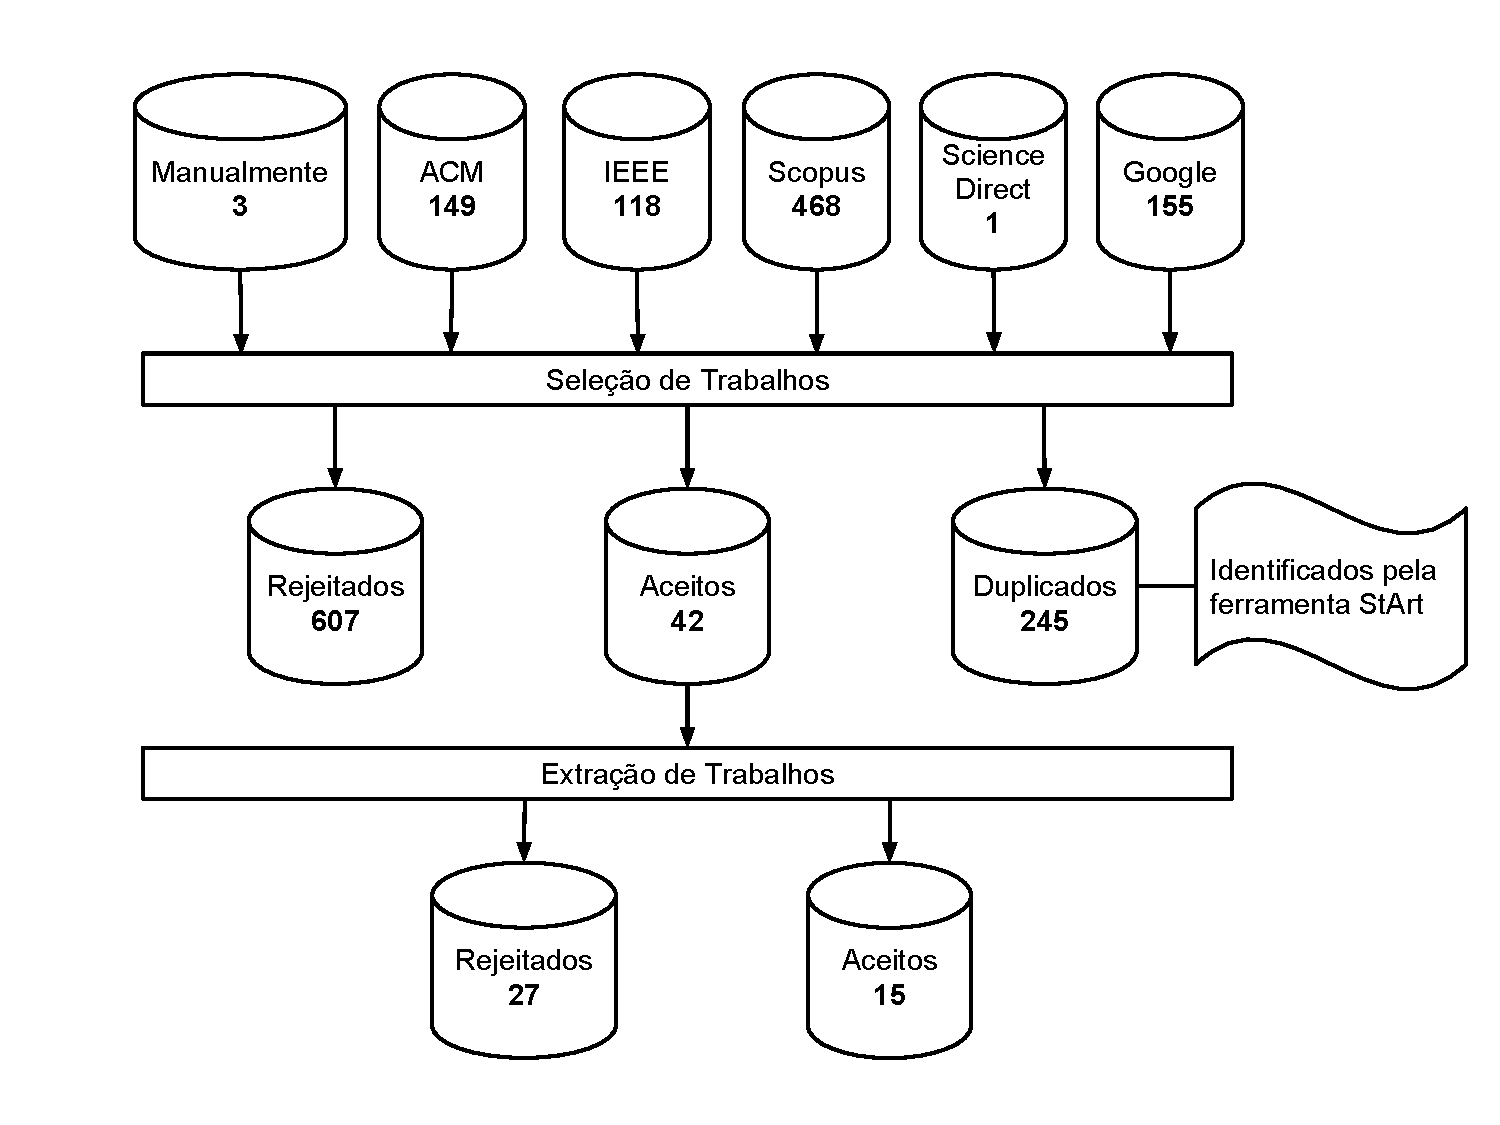
\includegraphics[scale=0.6]{figs/resultadosRevisao.pdf}}
    \end{center}
    \caption{Processo de seleção de trabalhos relevantes.}
    \label{fundamentacao:ageis:fatores:revisao}
\end{figure}

Finalmente, dentre os 15 trabalhos selecionados, foram identificados 20 fatores que influenciam a qualidade do TE em equipes ágeis. Esses fatores estão descritos na Tabela \ref{fundamentacao:ageis:fatores:tabela}.


\begin{table}[H]
\centering
\caption{Fatores-Chave que Influenciam a Qualidade do TE em Projetos Ágeis.}
\label{fundamentacao:ageis:fatores:tabela}
\resizebox{\textwidth}{!}{\begin{tabular}{|c|l|c|}
\hline
\textbf{Fator}                                                                            & \multicolumn{1}{c|}{\textbf{Conceito}}                                                                                                                                                                                                                                                        & \textbf{Referência}                                                                                                                                        \\ \hline
Comunicação                                                                               & Compartilhamento de informações entre os membros da equipe.                                                                                                                                                                                                                                   & \begin{tabular}[c]{@{}c@{}}\cite{hoegl} \cite{moe2} \cite{weimar} \cite{kozak}\\ \cite{schmidt} \cite{cockburn}\cite{gurram} \cite{johansson}\end{tabular} \\ \hline
Coordenação                                                                               & \begin{tabular}[c]{@{}l@{}}Refere-se à execução das atividades por parte dos integrantes da equipe\\ de maneira sincronizada e integrada.\end{tabular}                                                                                                                                        & \begin{tabular}[c]{@{}c@{}}\cite{hoegl} \cite{moe2} \cite{weimar} \cite{schmidt}\\ \cite{gurram}\end{tabular}                                              \\ \hline
Coesão                                                                                    & \begin{tabular}[c]{@{}l@{}}Atração interpessoal dos membros da equipe, seu compromisso com as tarefas \\ da equipe, e espírito de grupo.\end{tabular}                                                                                                                                         & \cite{hoegl} \cite{weimar} \cite{schmidt}                                                                                                                  \\ \hline
Confiança                                                                                 & \begin{tabular}[c]{@{}l@{}}A vontade de uma das partes ser vulnerável às ações de outra parte com base\\ na expectativa de que o outro irá executar uma determinada ação importante\\ para o cedente, independentemente da capacidade de monitorar ou controlar\\ a outra parte.\end{tabular} & \cite{weimar} \cite{schmidt} \cite{cockburn} \cite{tjornehoj}                                                                                              \\ \hline
\begin{tabular}[c]{@{}c@{}}Cooperação/\\ Colaboração/\\ Suporte Mútuo\end{tabular}        & \begin{tabular}[c]{@{}l@{}}Refere-se ao conceito de compromisso por parte do time como um todo\\ para alcançar os objetivos em comum.\end{tabular}                                                                                                                                            & \cite{hoegl} \cite{weimar} \cite{cockburn} \cite{johansson}                                                                                                \\ \hline
Diversidade de Valor                                                                      & Os membros da equipe compartilham dos mesmos valores e objetivos.                                                                                                                                                                                                                             & \cite{weimar}                                                                                                                                              \\ \hline
Liderança Compartilhada                                                                   & Autoridade na tomada de decisões e liderança deve ser compartilhada.                                                                                                                                                                                                                          & \begin{tabular}[c]{@{}c@{}}\cite{moe2} \cite{moe} \cite{schmidt} \cite{haraldsen}\\ \cite{ringstad} \cite{gurram}\end{tabular}                             \\ \hline
Orientação da Equipe                                                                      & Refere-se ao respeito mútuo entre os membros da equipe                                                                                                                                                                                                                                        & \begin{tabular}[c]{@{}c@{}}\cite{moe2} \cite{moe} \cite{stray} \cite{kozak}\\ \cite{haraldsen} \cite{ringstad} \cite{gurram}\end{tabular}                  \\ \hline
Redundância                                                                               & \begin{tabular}[c]{@{}l@{}}Capacidade dos membros da equipe poderem substituir uns aos outros \\ na realização das atividades sem a necessidade de treinamento.\end{tabular}                                                                                                                  & \cite{moe2} \cite{moe} \cite{kozak} \cite{haraldsen}                                                                                                       \\ \hline
Autonomia da Equipe                                                                       & \begin{tabular}[c]{@{}l@{}}Refere-se à influência de agentes externos a equipe na realização das\\ atividades da equipe.\end{tabular}                                                                                                                                                         & \cite{moe} \cite{ringstad} \cite{gurram}                                                                                                                   \\ \hline
\begin{tabular}[c]{@{}c@{}}Aprendizagem da Equipe/\\ Adaptabilidade\end{tabular}          & \begin{tabular}[c]{@{}l@{}}Habilidade de identificar mudanças no ambiente da equipe e ajustar as\\ estratégias de acordo com o necessário.\end{tabular}                                                                                                                                       & \begin{tabular}[c]{@{}c@{}}\cite{moe} \cite{stray} \cite{schmidt}\\ \cite{haraldsen} \cite{ringstad} \cite{gurram}\end{tabular}                            \\ \hline
Monitoramento                                                                             & Sincronização da equipe com relação às atividades e problemas.                                                                                                                                                                                                                                & \cite{moe2} \cite{haraldsen} \cite{gurram}                                                                                                                 \\ \hline
\textit{Feedback}                                                                         & \begin{tabular}[c]{@{}l@{}}Refere-se ao ato de prover, encaminhar e receber informações\\ relacionadas ao desempenho dos membros da equipe.\end{tabular}                                                                                                                                      & \cite{moe2} \cite{gurram}                                                                                                                                  \\ \hline
Cultura                                                                                   & \begin{tabular}[c]{@{}l@{}}Conjunto de experiências, compreensões e significados compartilhados\\ entre os membros da equipe.\end{tabular}                                                                                                                                                    & \cite{kozak}                                                                                                                                               \\ \hline
Personalidade                                                                             & Personalidade dos indivíduos que compõem a equipe.                                                                                                                                                                                                                                            & \cite{lalsing} \cite{kozak} \cite{schmidt}                                                                                                                 \\ \hline
Distribuição da Equipe                                                                    & A distribuição física da equipe.                                                                                                                                                                                                                                                              & \cite{lalsing}                                                                                                                                             \\ \hline
Tamanho da Equipe                                                                         & A quantidade de pessoas na equipe.                                                                                                                                                                                                                                                            & \cite{lalsing}                                                                                                                                             \\ \hline
\begin{tabular}[c]{@{}c@{}}Balanço das Contribuições\\ dos Membros da Equipe\end{tabular} & \begin{tabular}[c]{@{}l@{}}A capacidade de todos os membros da equipe contribuírem com todo\\ o conhecimento necessário para o desenvolvimento das atividades.\end{tabular}                                                                                                                   & \cite{hoegl}                                                                                                                                               \\ \hline
Esforço                                                                                   & \begin{tabular}[c]{@{}l@{}}Compartilhamento da carga de trabalho e priorização das tarefas da equipe\\ em relação a outras obrigações são indicadores do esforço de membros\\ da equipe para exercer as tarefas em comum.\end{tabular}                                                        & \cite{hoegl}                                                                                                                                               \\ \hline
Motivação                                                                                 & \begin{tabular}[c]{@{}l@{}}Motivação dos membros da equipe para realizar as atividades e trabalhar\\ em grupo.\end{tabular}                                                                                                                                                                   & \cite{whitworth}                                                                                                                                           \\ \hline

\end{tabular}}
\end{table}


A \textit{Comparative Agility}\footnote{\url{https://comparativeagility.com/}} é uma ferramenta \textit{web} quer permite avaliar o quão ágil uma organização é em relação à outras. De acordo com o site, essa ferramenta é considerada a mais abrangente em relação à avaliação ágil na indústria. Essa avaliação é feita com base em um \textit{survey online} organizado em sete dimensões e trinta e duas características. Uma das dimensões consideradas nessa ferramenta é o \textit{Trabalho em Equipe}. Essa dimensão é dividida em três características (i.e., Composição da Equipe, Gerenciamento e Comunicação). Para cada uma dessas características, há perguntas relacionadas a fatores que influenciam essas características. A Figura \ref{fundamentacao:ageis:fatores:comparativeagility} representa o relacionamento entre a dimensão \textit{Trabalho em Equipe}, suas características e os aspectos que contribuem para a boa qualidade dessas características.

\begin{figure}[H]
\begin{center}
        \fbox{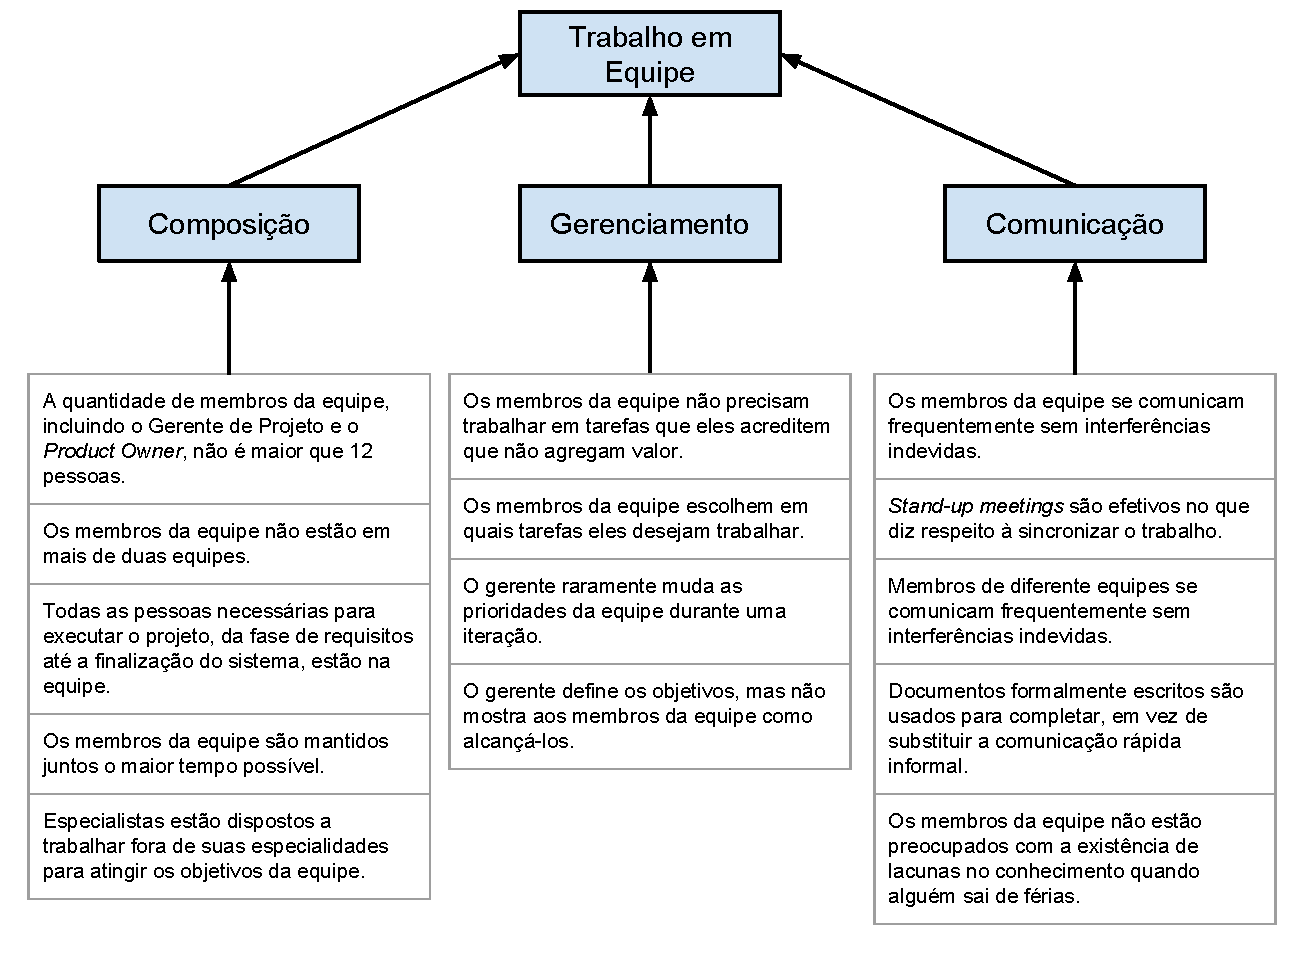
\includegraphics[scale=0.67]{figs/comparativeAgility_teamwork.pdf}}
    \end{center}
    \caption{Representação do Trabalho em Equipe na Ferramenta \textit{Comparative Agility}.}
    \label{fundamentacao:ageis:fatores:comparativeagility}
\end{figure}

\section{Redes Bayesianas}
\label{fundamentacao:redes}

Redes Bayesianas vêm sendo bastante utilizadas para formular soluções de problemas reais que envolvem risco. Alguns exemplos são:

\begin{itemize}
  \item Segurança de sistemas embarcados na indústria ferroviária \cite{neil};
  \item Confiabilidade de veículos militares \cite{neil2};
  \item Risco de colisões no tráfego aéreo \cite{neil3};
  \item Predição de defeitos de \textit{software} em produtos eletrônicos \cite{neil4} \cite{fenton2} \cite{fenton3} \cite{fenton4};
  \item Identificação de falhas em projetos de desenvolvimento de \textit{software} \cite{perkusich2013} \cite{perkusich2014}.
\end{itemize}

Segundo Neapolitan et al. \cite{neapolitan}, a técnica de RB surgiu para representar contextos em que há um grande número de variáveis, e o objetivo de verificar a influência probabilística que uma ou mais variáveis exercem sobre outras. Assim, mesclando princípios de Teoria dos Grafos, Probabilidade, Ciência da Computação e Estatística, a utilização de RB permite representar e avaliar contextos como os supracitados \cite{bengal}.

Portanto, RB pertencem à família de modelos gráficos pobabilísticos e são utilizados para representar incertezas de um domínio \cite{bengal}. Em virtude da subjetividade envolvendo os conceitos explorados neste trabalho, decidiu-se utilizar essa técnica para representar as incertezas associadas a eles.

De maneira formal, uma Rede Bayesiana, $B$, pode se representada pela tupla \{$G$, $\Theta$\}, onde $G$ é um Grafo Acíclico Dirigido (GAD) e $\Theta$ o conjunto de parâmetros que quantificam a rede. No GAD $G$, o conjunto de nós $V = X1, \ldots,Xn$ representa as varáveis aleatórias, e os arcos representam dependências diretas entre essas variáveis. O conjunto $\Theta$ contém o parâmetro $\theta_{x_{i}|\pi_{i}} = P_{B}(x_{i}|\pi_{i})$ para cada $x_{i}$ (i.e., estado possível) em $X_{i}$, onde $\pi_{i}$ representa os estados dos pais $X_{i}$ no GAD $G$. A Equação \ref{fundamentacao:redes:eq} representa a distribuição de probabilidade conjunta definida por $B$ sobre o conjunto $V$.

\begin{equation}\label{fundamentacao:redes:eq}
  P_{B}(X_{1}, \ldots, X_{n}) = \prod\limits_{i=1}^n P_{B}(x_{i}|\pi_{i}) = \prod\limits_{i=1}^n \theta_{X_{i}|\pi{i}}
\end{equation}

Na Figura \ref{fundamentacao:redes:exemplo} é apresentada uma RB. Os círculos representam os nós e as setas representam os arcos. As Tabelas de Probabilidade dos Nós (TPN) são apresentadas ao lado de cada um dos nós. Apesar da direção dos arcos representarem uma conexão casual entre os nós, a informação pode propagar em qualquer direção \cite{pearl}.

\begin{figure}[H]
\begin{center}
        \fbox{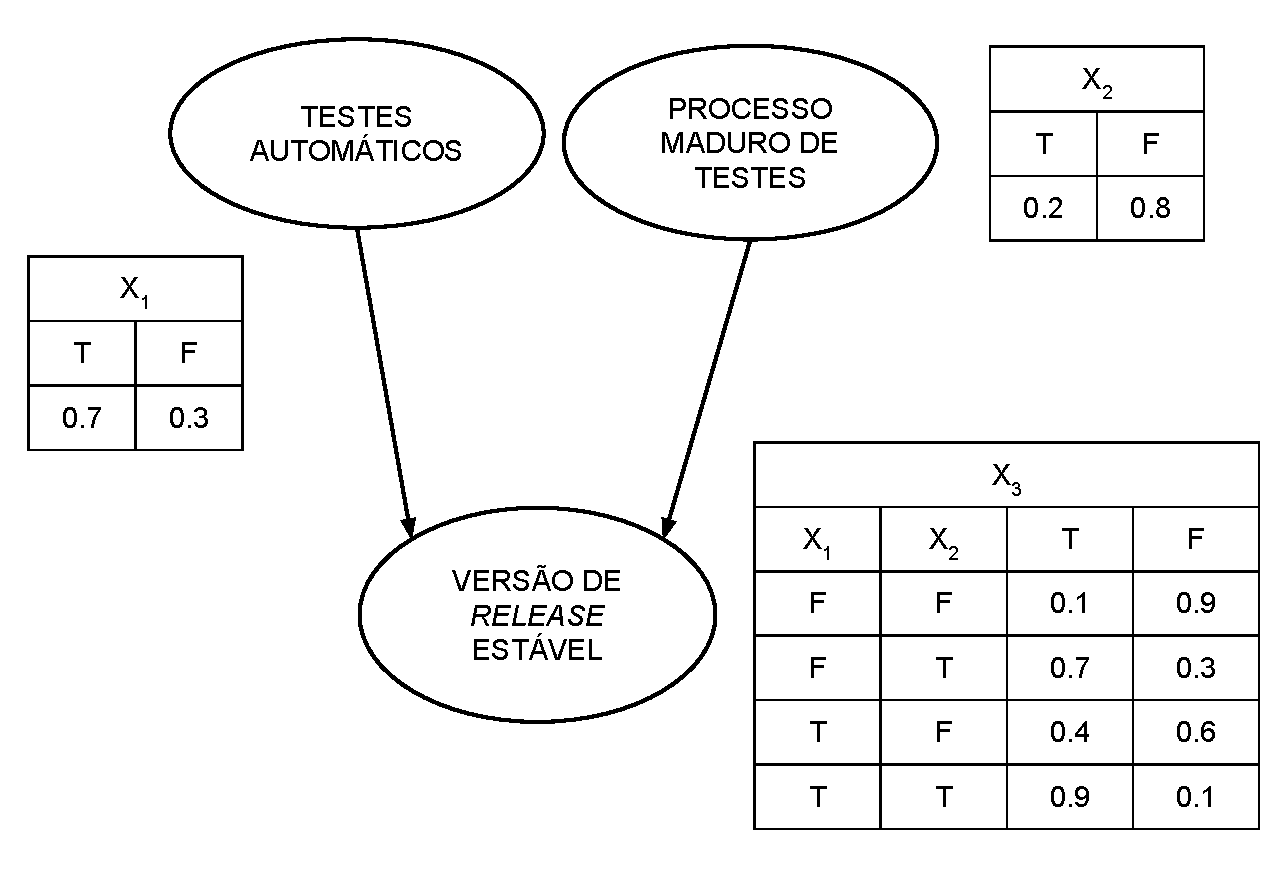
\includegraphics[scale=0.67]{figs/BN-Exemplo.pdf}}
    \end{center}
    \caption{Exemplo de Rede Bayesiana.}
    \label{fundamentacao:redes:exemplo}
\end{figure}

\subsection{Construção de Redes Bayesianas}
\label{fundamentacao:redes:construcao}

A construção de uma RB pode ser dividida em duas etapas: a construção do GAD e a definição das tabelas de probabilidade.

\subsubsection{Construção do GAD}
\label{fundamentacao:redes:construcao:gad}

Cada nó do GAD, neste trabalho, representa um fator que influencia a qualidade do TE e há um arco entre dois nós sempre houver um relação direta entre ele dois. Esse arco está direcionado para o nó influenciado na relação. Além disso, cada fator chave possui uma quantidade de estados possíveis, além uma probabilidade associada a cada estado. Assim, conforme apresentado em \cite{perkusich2013}, cada nó representa um conjunto de tuplas $N = \{(s_{1},p_{1}), \ldots, (s_{\left|{N}\right|},p_{\left|{N}\right|})\}$, onde $s_{i}$ é um estado possível do nó e $p_{i}$ é a probabilidade associada a esse estado. O conjunto de fatores-chave é apresentado como $F = \{N_{1}, \ldots, N_{\left|{F}\right|}\}$. O conjunto de arcos, por sua vez, é apresentado como $R = \{(N_{j},N_{k}) \mid N_{j} \subset F \wedge N_{k} \subset F\}$, onde $N_{j}$ é ponto inicial do arco e $N_{k}$ o ponto final

Portanto, para concluir a primeira etapa da construção de uma RB, deve-se encontrar todos os elementos dos conjuntos $F$ e $R$. Para encontrar todos os elementos de $F$, é necessário identificar os fatores-chave $N_{a}$ e, para cada um desses fatores, todos os seus possíveis estados $s_{i}$ e probabilidades associadas $p_{i}$, onde $a \le \left|{F}\right|$ e $i \le \left|{N_{a}}\right|$. Finalmente, para encontrar todos os elementos do conjunto $R$, é necessário identificar todas $f_{j}$ e $f_{k}$, onde $f_{j}$ e $f_{k}$ $\in F$.

Dessa forma, pode-se dividir a etapa de construção do DAG em dois sub-problemas: identificar os elementos de $F$ e $R$, e identificar os elementos de $N$. Assim, esse primeiro sub-problema desta etapa diz respeito à identificação desses fatores e os relacionamentos entre eles. No segundo sub-problema, a preocupação deve ser focada em identificar os possíveis estados, além de suas probabilidades, para cada nó do GAD.

\subsubsection{Definição das Tabelas de Probabilidade}
\label{fundamentacao:redes:construcao:funcoes}

Apesar de RB serem úteis para resolverem problemas reais relacionados com risco e subjetividade, o seu uso ainda é restrito devido a dificuldade em definir as TPN. Há duas maneiras de se coletar dados para definir as TPN de uma RB: base de dados ou opinião de especialistas. Contudo, não é fácil encontrar uma base de dados adequada para um cenário específico de um problema prático. Por outro lado, a definição das TPN com a ajuda de especialistas requer bastante esforço (e.g., definir TPN para nós com um número muito alto de estados ou alta quantidade de pais, pois a quantidade de linhas de uma TPN aumenta exponencialmente em função da quantidade de pais do nó em questão). De acordo com Fenton et al. \cite{fenton}, isso pode acarretar em vários tipos de inconsistências no modelo.

Há vários métodos que têm como objetivo diminuir a complexidade e codificar a experiência de especialistas em grandes TPN. Noisy-OR \cite{huang} e Noisy-MAX \cite{diez} são dois exemplos desses métodos. Contudo, Noisy-OR só pode ser aplicado a nós booleanos, e Noisy-MAX não é capaz de modelar o intervalo de relacionamentos que precisamos neste trabalho. Das \cite{das} propôs um algoritmo para popular as TPN que visa diminuir o tempo de duração para adquirir conhecimento de especialistas. Perkusich et al. \cite{perkusichNPT}, por sua vez, propõem um algoritmo cujo objetivo é ordenar os nós pai com base em sua relevância para o nó filho. Em seguida, com os nós pai ordenados por ordem de relevância, deve-se gerar as funções ponderadas com base na relevância dos nós pais e, finalmente, aplicá-las como funções de probabilidade dos nós.

Por outro lado, Fenton et al. \cite{fenton} propõem uma abordagem que utiliza Nós Ranqueados (NR). Essa abordagem é baseada numa distribuição normal duplamente truncada (TNormal) que usa como média um tipo de função ponderada em função dos valores dos nós pai. Essa distribuição é baseada em quatro parâmetros: $u$, média (i.e., tendência central); $\sigma^{2}$, variância (i.e., confiança dos resultados); $a$, limite inferior (i.e., 0); e $b$, limite superior (i.e., 1). Essa distribuição permite que quem a utilize modele uma varidade de formas (i.e., relacionamentos). Por exemplo: uma distribuição uniforme ($\sigma^{2} = \infty$) e distribuições muito enviesadas ($\sigma^{2} = 0$). Na Figura \ref{fundamentacao:redes:construcao:funcoes:tnormal} há alguns exemplos de funções TNormal.

\begin{figure}[ht!]
\begin{center}
		\fbox{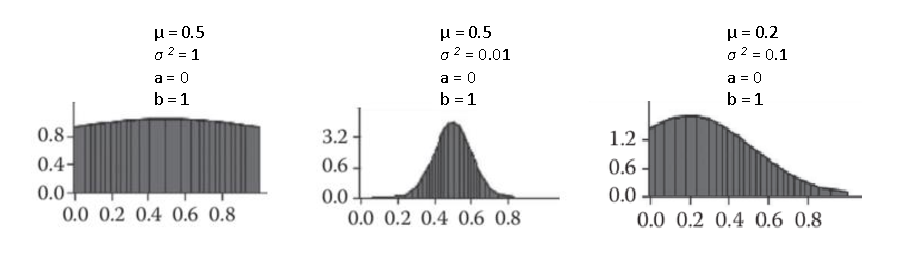
\includegraphics[scale=1]{figs/tnormalExemplos.pdf}}
	\end{center}
	\caption{Exemplos de Funções TNormal.}
	\label{fundamentacao:redes:construcao:funcoes:tnormal}
\end{figure}

Nessa abordagem, $u$ é definido por uma função ponderada baseada nos nós pai. Existem quatro tipos de funções ponderadas: média ponderada (WMEAN), mínimo ponderada (WMIN), máximo ponderada (WMAX) e uma última função que mescla a WMIN e a WMAX (MIXMINMAX). De acordo com os autores, essas funções são suficientes para representar os tipos de relações necessárias para definir as TPN. A Figura \ref{fundamentacao:redes:construcao:funcoes:ponderadas} contém exemplos de TPN calculadas com essas funções. Entretanto, apesar de WMEAN e MIXMINMAX apresentarem os mesmos valores, há uma diferença entre elas. A função WMEAN calcula a média ponderada dos nós pai, baseado nos pesos de cada nó pai, e a função MIXMINMAX mescla as funções WMIN e WMAX, também baseado nos pesos dos nós pai.

\begin{figure}[ht!]
\begin{center}
		\fbox{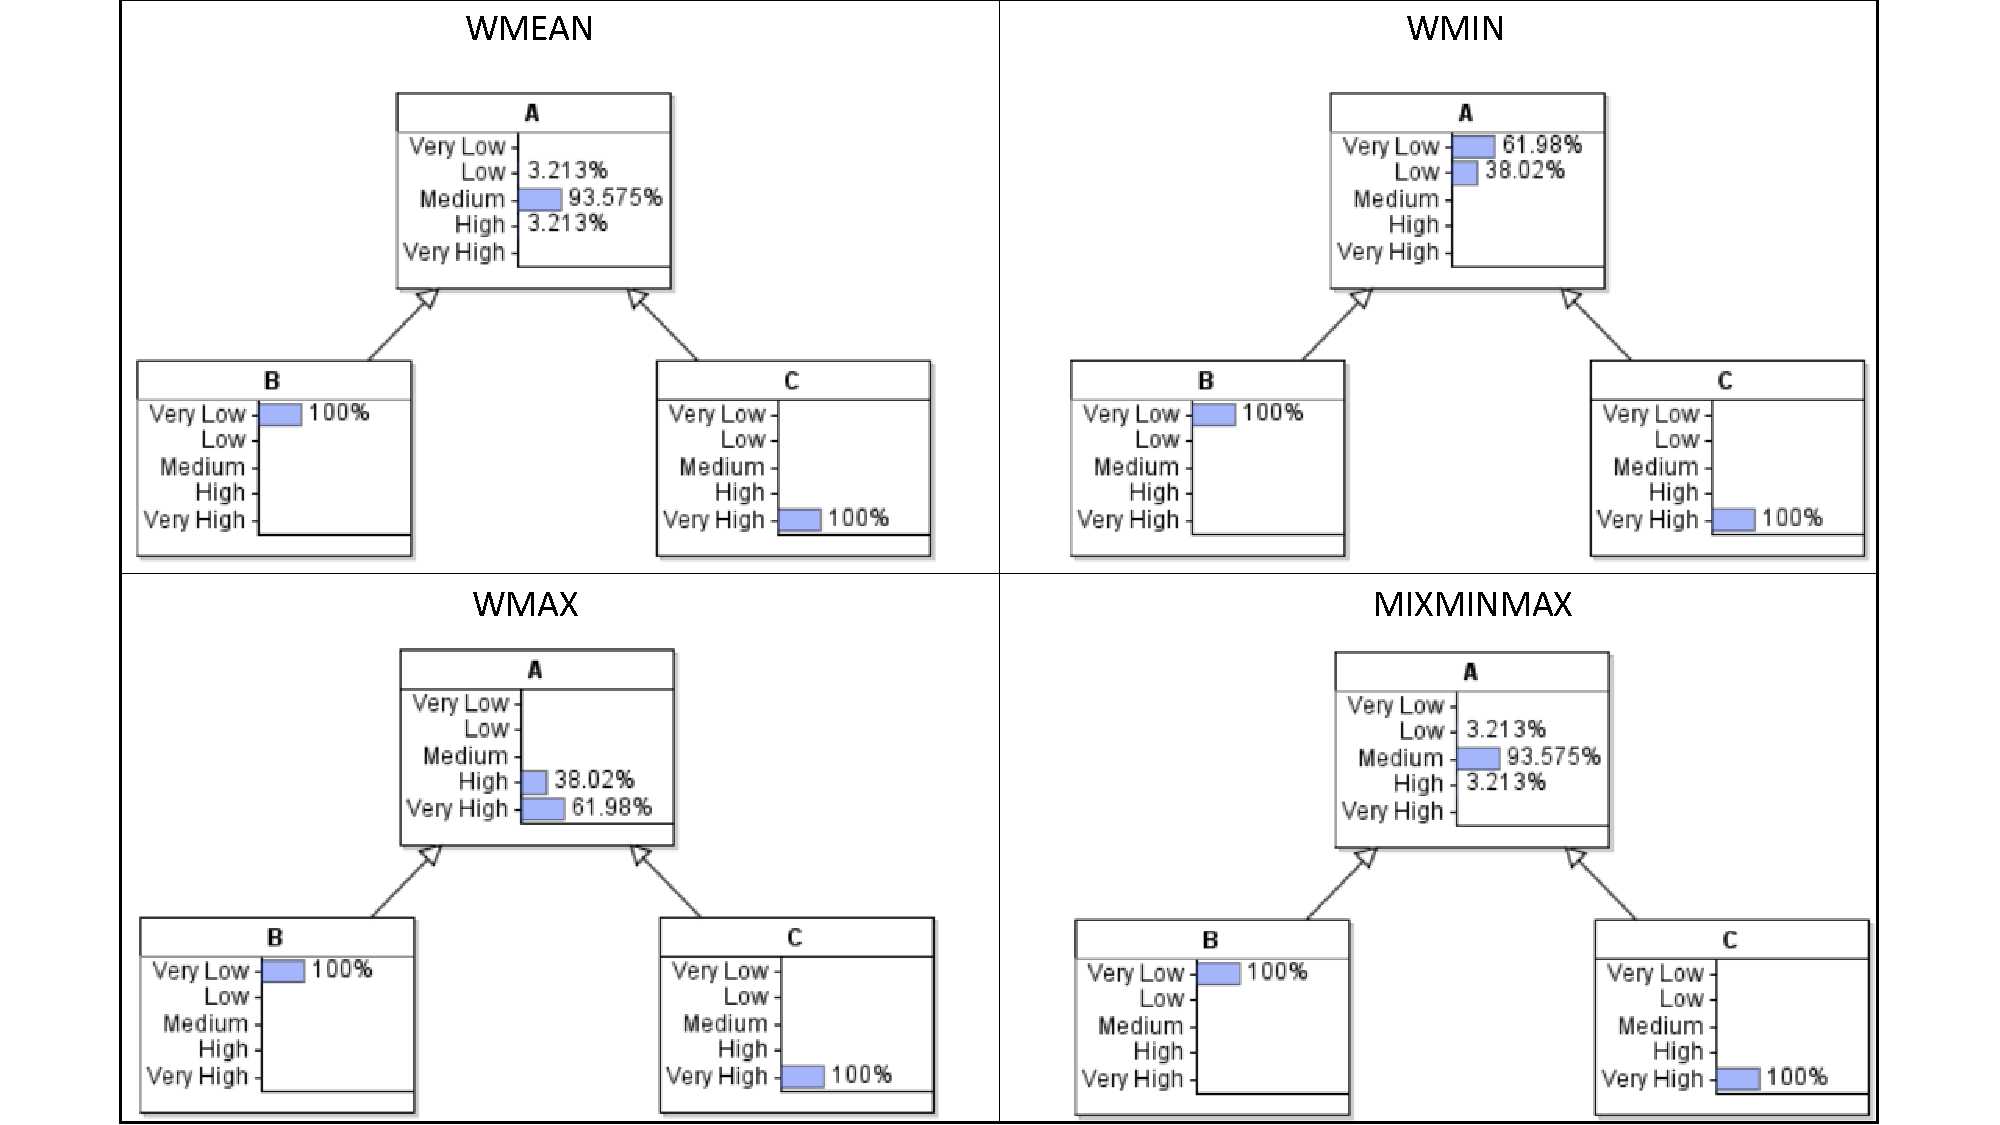
\includegraphics[scale=0.47]{figs/funcoesExemplos.pdf}}
	\end{center}
	\caption{Exemplos das Funções Ponderadas.}
	\label{fundamentacao:redes:construcao:funcoes:ponderadas}
\end{figure}

Para definir qual função deve ser utilizada, o indivíduo que está construindo o modelo deve definir perguntas para coletar respostas e definir as TPN. Tomando como base a RB representada na Figura \ref{fundamentacao:redes:construcao:funcoes:bn1}, um exemplo de pergunta seria: "Se o estado do nó X1 for Muito Alto e o estado do nó X2 for Muito Baixo, qual o valor esperado para o nó Y?". Baseado nas respostas, o indivíduo que está construindo a RB deve definir qual a função e quais os pesos adequados para definir as TPN. A variância deve ser definida empiricamente e deve refletir a confiança dos especialistas nos resultados.

\begin{figure}[ht!]
\begin{center}
		\fbox{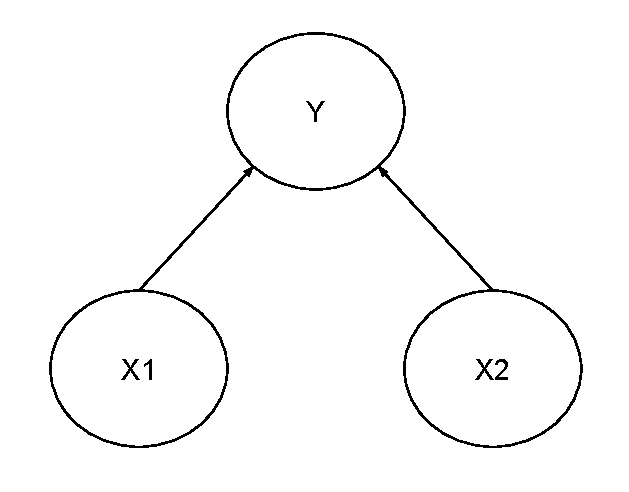
\includegraphics[scale=0.8]{figs/BN-2nos.pdf}}
	\end{center}
	\caption{Exemplo de Nó Filho com Dois Pais.}
	\label{fundamentacao:redes:construcao:funcoes:bn1}
\end{figure}

Entretanto, a base da abordagem proposta em \cite{fenton} consiste em mapear os estados dos nós em uma escala numérica. Logo, quanto menos precisa a tendência central do nó filho, mais vaga será a distribuição da função atribuida. Como forma de mitigar esses problemas, em \cite{laitila} é proposta uma abordagem similar. Contudo, nessa abordagem, em vez do especialista avaliar a função de probabilidade de um determinado nó filho atribuindo a qual dos estados desse nó a tendência central corresponde, são atríbuidas probabilidades para cada um dos estados do nó filho - a soma dessas probabilidades deve ser igual a 1. De acordo com o autor, essa abordagem provê uma transparência maior na elicitação dos pesos dos nós pai na função ponderada.
